\chapter{Background}
\label{chap:background}

This section describes the theoretical concepts of importance for the thesis along with the specifics of scaling agile in the organisation under study.

\section{Conceptual Background}

This subsection presents the primary concepts the researchers operate throughout the study: it explains information and communication and the difference between the two and presents the notions of heat maps and social networks.

\subsection{Communication \& Information}
\label{chap:background-comm-info}

Communication is the exchange of meaning between various parties. Within this exchange, the medium's specific channel type or physical nature to exchange meaning is not of interest in most theories~\citep{savage2011informationtheory}.~\citet{shannon1948theoryofcommunication}, as illustrated in Figure \ref{fig:communication-system}, defines a model which envisions the role of a transmitter and receiver between which the signal is transferred while being prone to potential external noise. Internal noise, on the other hand, can emerge during the encoding or decoding process of a sender or receiver~\citep{verdu1998informationtheory}.
In addition, messages are exposed to an exponentially increasing amount of noise in relation to the nodes they pass through. This specially applies for large organisations with long distances between the sender and final receiver~\citep{shannon1948theoryofcommunication}.

\begin{figure}[h!]
  \centering
  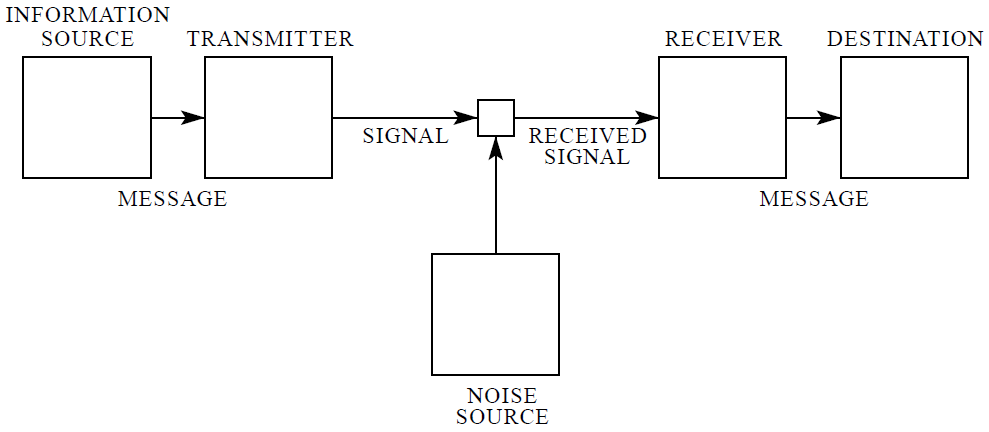
\includegraphics[width=0.90\textwidth]{figures/communication-information-shannon.png}
  \caption{Schematic diagram of a general communication system~\citep{shannon1948theoryofcommunication}}
  \label{fig:communication-system}
\end{figure}

Information coheres to communication as it is perceived as the message which travels between parties~\citep{floridiinformationintro}. Just as~\citet{savage2011informationtheory} attempts to embed communication in a mathematical model, information theory formalises areas of signal processing and data compression. Signals are not independent of their context and static in how they are understood during interpretation before their transmission~\citep{vigo2011representionalinformation}. Whenever a single piece of information is accessed, a human processes it, which is a dynamic procedure strongly influenced by the context of the actor and its ability to understand the information's complexity~\citep{vigo2011representionalinformation}. Finally, whenever the meaning conveyed constitutes something previously unknown,~\citet{gleick2012theinformation} acknowledges actual information being transmitted.

In the scope of this thesis the concepts linked to information and communication are being handled separately. \textit{Communication} is understood as a form of humans dynamically exchanging information through various channels where \textit{information} is a single manifestation of a message's content.

\subsection{Heat Maps}

Heat maps were first used over a century ago to illustrate social statistics across various districts in France~\citep{friendly09thehistory}. 
Over time statisticians have worked on different algorithms to perform various types of clusterings involving permutations of the heat maps' rows and columns~\citep{friendly09thehistory}, allowing the heat map to be more powerful visualisation tool communicating the data's statement clearly.
As a result, heat maps are often used to visualise dense, three-dimensional data of a table format. Data in regards to an observation can be collected continuously over or at a discrete point in time~\citep{gehlensborg2012heatmaps}.
Colour coding is then used to give structure and illustrate clusterings. All in all, it allows for an easier interpretation of the original data~\citep{gehlensborg2012heatmaps}. Their data independence allows heat maps to be applied in different fields such as social science, biology or meteorology.

In software engineering~\citet{feldt2013heatmaps} use heat maps to visualize code churns over time of different code elements to predict potential integration problems. Other investigations visualize the change status with a file and project view using colour coding for each line's status~\citep{voinea2007visualassessment}. The aggregated project view gives a dense view of the overall status also linking progress to single developers.
\citet{coplien1996patternsofprod} utilise heat maps to visualise the intensity of communication between roles within software development organisations. Their heat maps, which are called interaction grids, are sorted in descending order according to the roles' communication intensities, illustrating the epicentre of communication and the associated roles at the point of origin. By performing further analysis and data comparisons,~\citet{coplien1996patternsofprod} deduct characteristics of successful corporations such as inward communication flow, even distribution of work and the distribution of communication among roles.

Heat maps are used in the context of this thesis to demonstrate the intensities of communications of different natures between the representatives of various roles in an organisation.

\subsection{Social Networks}

Social networks are a concept vastly used in sociology as a mean to represent social groups as networks of their interrelations. Their analysis has been mathematically formalised and, as outlined by \citet{scott2011sn}, is closely related to the methods of graph theory. Using the terminology of the latter, individuals (or groups of individuals) in a social network are represented as nodes while their interrelations are depicted by edges. \citet{scott2011sn} mentions the measures of network density and centrality, examination of cliques and clusters as a few aspects of a social network that can be investigated using existing methods and theories.

Linguistics, criminology and demography are among other research areas that over time incorporated the analysis of social networks in their field of study. 

In software engineering's body of knowledge, social networks have been used for instance by \citet{Cataldo2008} for communication analysis in a geographically distributed software development to study the core of communication networks and the level of technical proficiency of those in the core. 

The thesis employs social networks to complement the heat maps visualisations with a structured overview of the communication paths between the representatives of various roles in an organisation.

\section{Agile at Ericsson within PDU LMR}

Increasing productivity remains the main purpose towards the application of agile methodologies in industry. Nevertheless,~\citet{badampudi2013proddelay} point out that most companies adapting agile do not manage to strictly follow all of its main ideas. Adjustments are made to integrate agile with the large scale and existing processes, with both positive and negative impacts upon productivity. Similarly, Ericsson has its own peculiarities of scaling agile which will be discussed in this section.

\subsection{History of the Transformation}

Dissatisfied with performance, several years ago the~\ac{PDU LMR} organisation at Ericsson started a transformation from the waterfall based development towards a more agile approach, following small incremental and discontinuous transformation steps. Rather than only changing the lower level coordination of development teams, it has been decided to change the organisational structure along the way. A matrix-like organisational structure was replaced with hierarchical one with~\acp{XFT} at its top trying to embrace agile software development: a structure not necessarily prescribed by agile but motivated by Ericsson's scale. The strictly hierarchical structure causes a lower number of connections, clear responsibilities and delegation but embodies potential queuing delays. 

This is justified by the fact that matrix structures in general and as previously employed by Ericsson, combine functional (divided by types of work) and divisional (product based division) structures, adding another horizontal line of communication~\citep{price2007hrm}. Hence, each unit within the structure is being coordinated by two superior entities: a functional- and a divisional superiority. The intent is to faster distribute knowledge horizontally among functional sectors without having to move through a long chain of hierarchies~\citep{galbraith2008matrix}. 
Hierarchical structures on the other hand are solely an extension to functional or divisional structures adding a chain of command and show superior and subordinate units or roles. The hierarchy does not imply horizontal communication and becomes narrower towards its top~\citep{healeyprojectmanagement}.

PDU LMR integrated parts of agile's methodologies into their hierarchical organisational structure while adding variations where needed. This includes partially deploying methodologies, defining custom roles and responsibilities, and adding an integration layer for the organisational structure.

\subsection{Organisational Structure at Ericsson PDU LMR}
\label{Chap:OrgStrucEricsson}

The structure of the organisation under study is presented on the Figure \ref{fig:org-structure}.

\begin{figure}[h!]
  \centering
  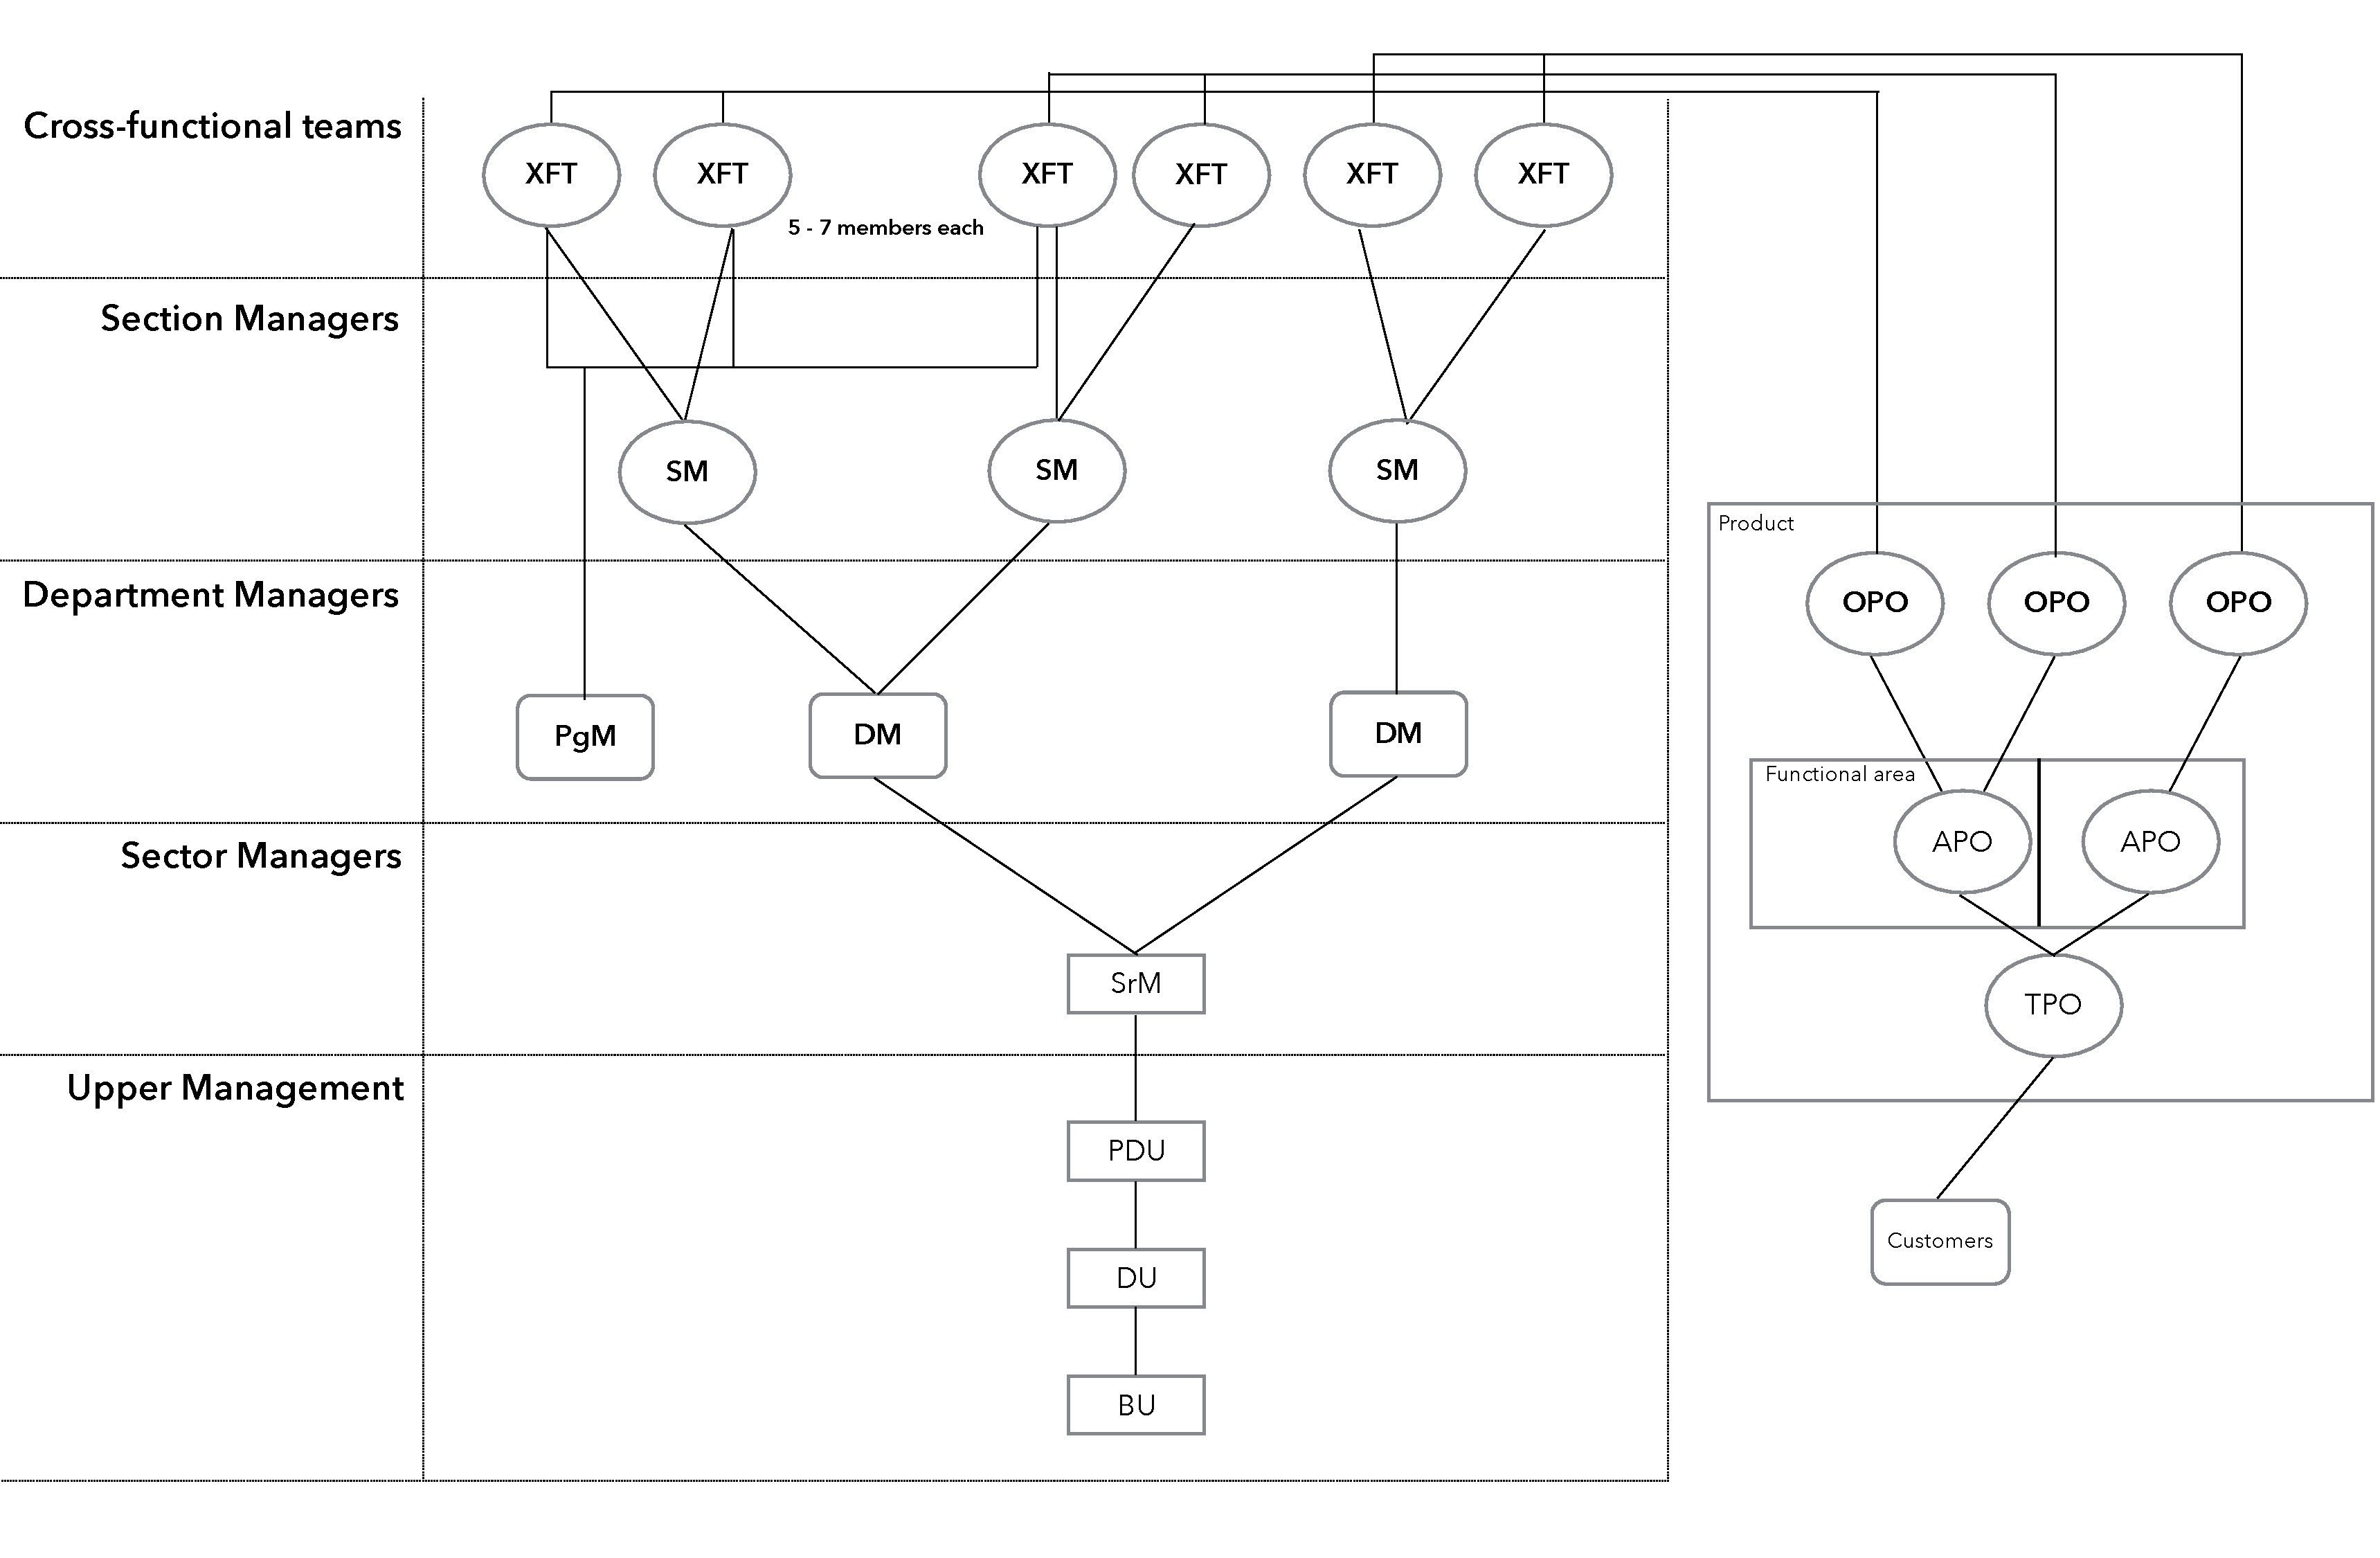
\includegraphics[width=0.90\textwidth]{figures/organisational-structure.pdf}
  \caption{Organisational structure of~\ac{PDU LMR}}
  \label{fig:org-structure}
\end{figure}

Roles with a strict relation to agile methodologies are illustrated with an ellipse and more thorough description of their responsibilities can be found in Table 3.1. Roles are grouped horizontally and the connecting lines outline the organisation's hierarchy and intended chain of commands.

In the epicentre of the development activities reside multiple~\acp{XFT} — self-sufficient units which have all the necessary competencies for feature delivery at their disposal.~\acp{XFT} generally consist of five to nine members. 
\acp{PG} are not part of an~\ac{XFT} but are also assigned to different products in order to oversee development and maintain a product's coherence.~\acp{XFT} working on parts of a whole product in turn interact with one or several~\acp{PG} which for teams also eases handling of its size and complexity.

Each team belongs to a section with a~\ac{SM} looking over two or more~\acp{XFT}. The~\ac{SM} also acts as a~\ac{TC}, whose responsibilities are described later in the Table 3.1.
Sections themselves belong to departments, which in turn are a part of a sector, each of them having a respective manager. A structure above the sector in the hierarchy is called a~\ac{PDU}. Together, this part of the structure constitutes the line organisation. The line is further supervised by a Design Unit (DU) and a Business Unit (BU) which are not part of further discussions.

The start of the transformation towards an agile development process caused the addition of a new product owner community to the existing structure (depicted on the right hand side of Figure~\ref{fig:org-structure}). Given the company's scale, the traditional role of a~\ac{PO} had to be divided into the areas of responsibility. Thus, new roles of~\acp{TPO},~\acp{APO} and~\acp{OPO} were introduced with a~\ac{TPO} being in direct contact with the customer and~\acp{APO}, who in turn work closely together with several~\acp{OPO} each.~\acp{OPO} themselves work with several~\acp{XFT} at a time. The exact amount depends on the nature of the product and a way of working inside a section. In case of a feature assigned to an \ac{XFT} being too large and complex, a~\ac{FPjM} acts as an intermediary between the~\ac{PgM} and~\acp{OPO}, where the former is responsible for maintaining the high-level backlogs teams eventually get the stories from.

\begin{figure}[h!]
  \centering
  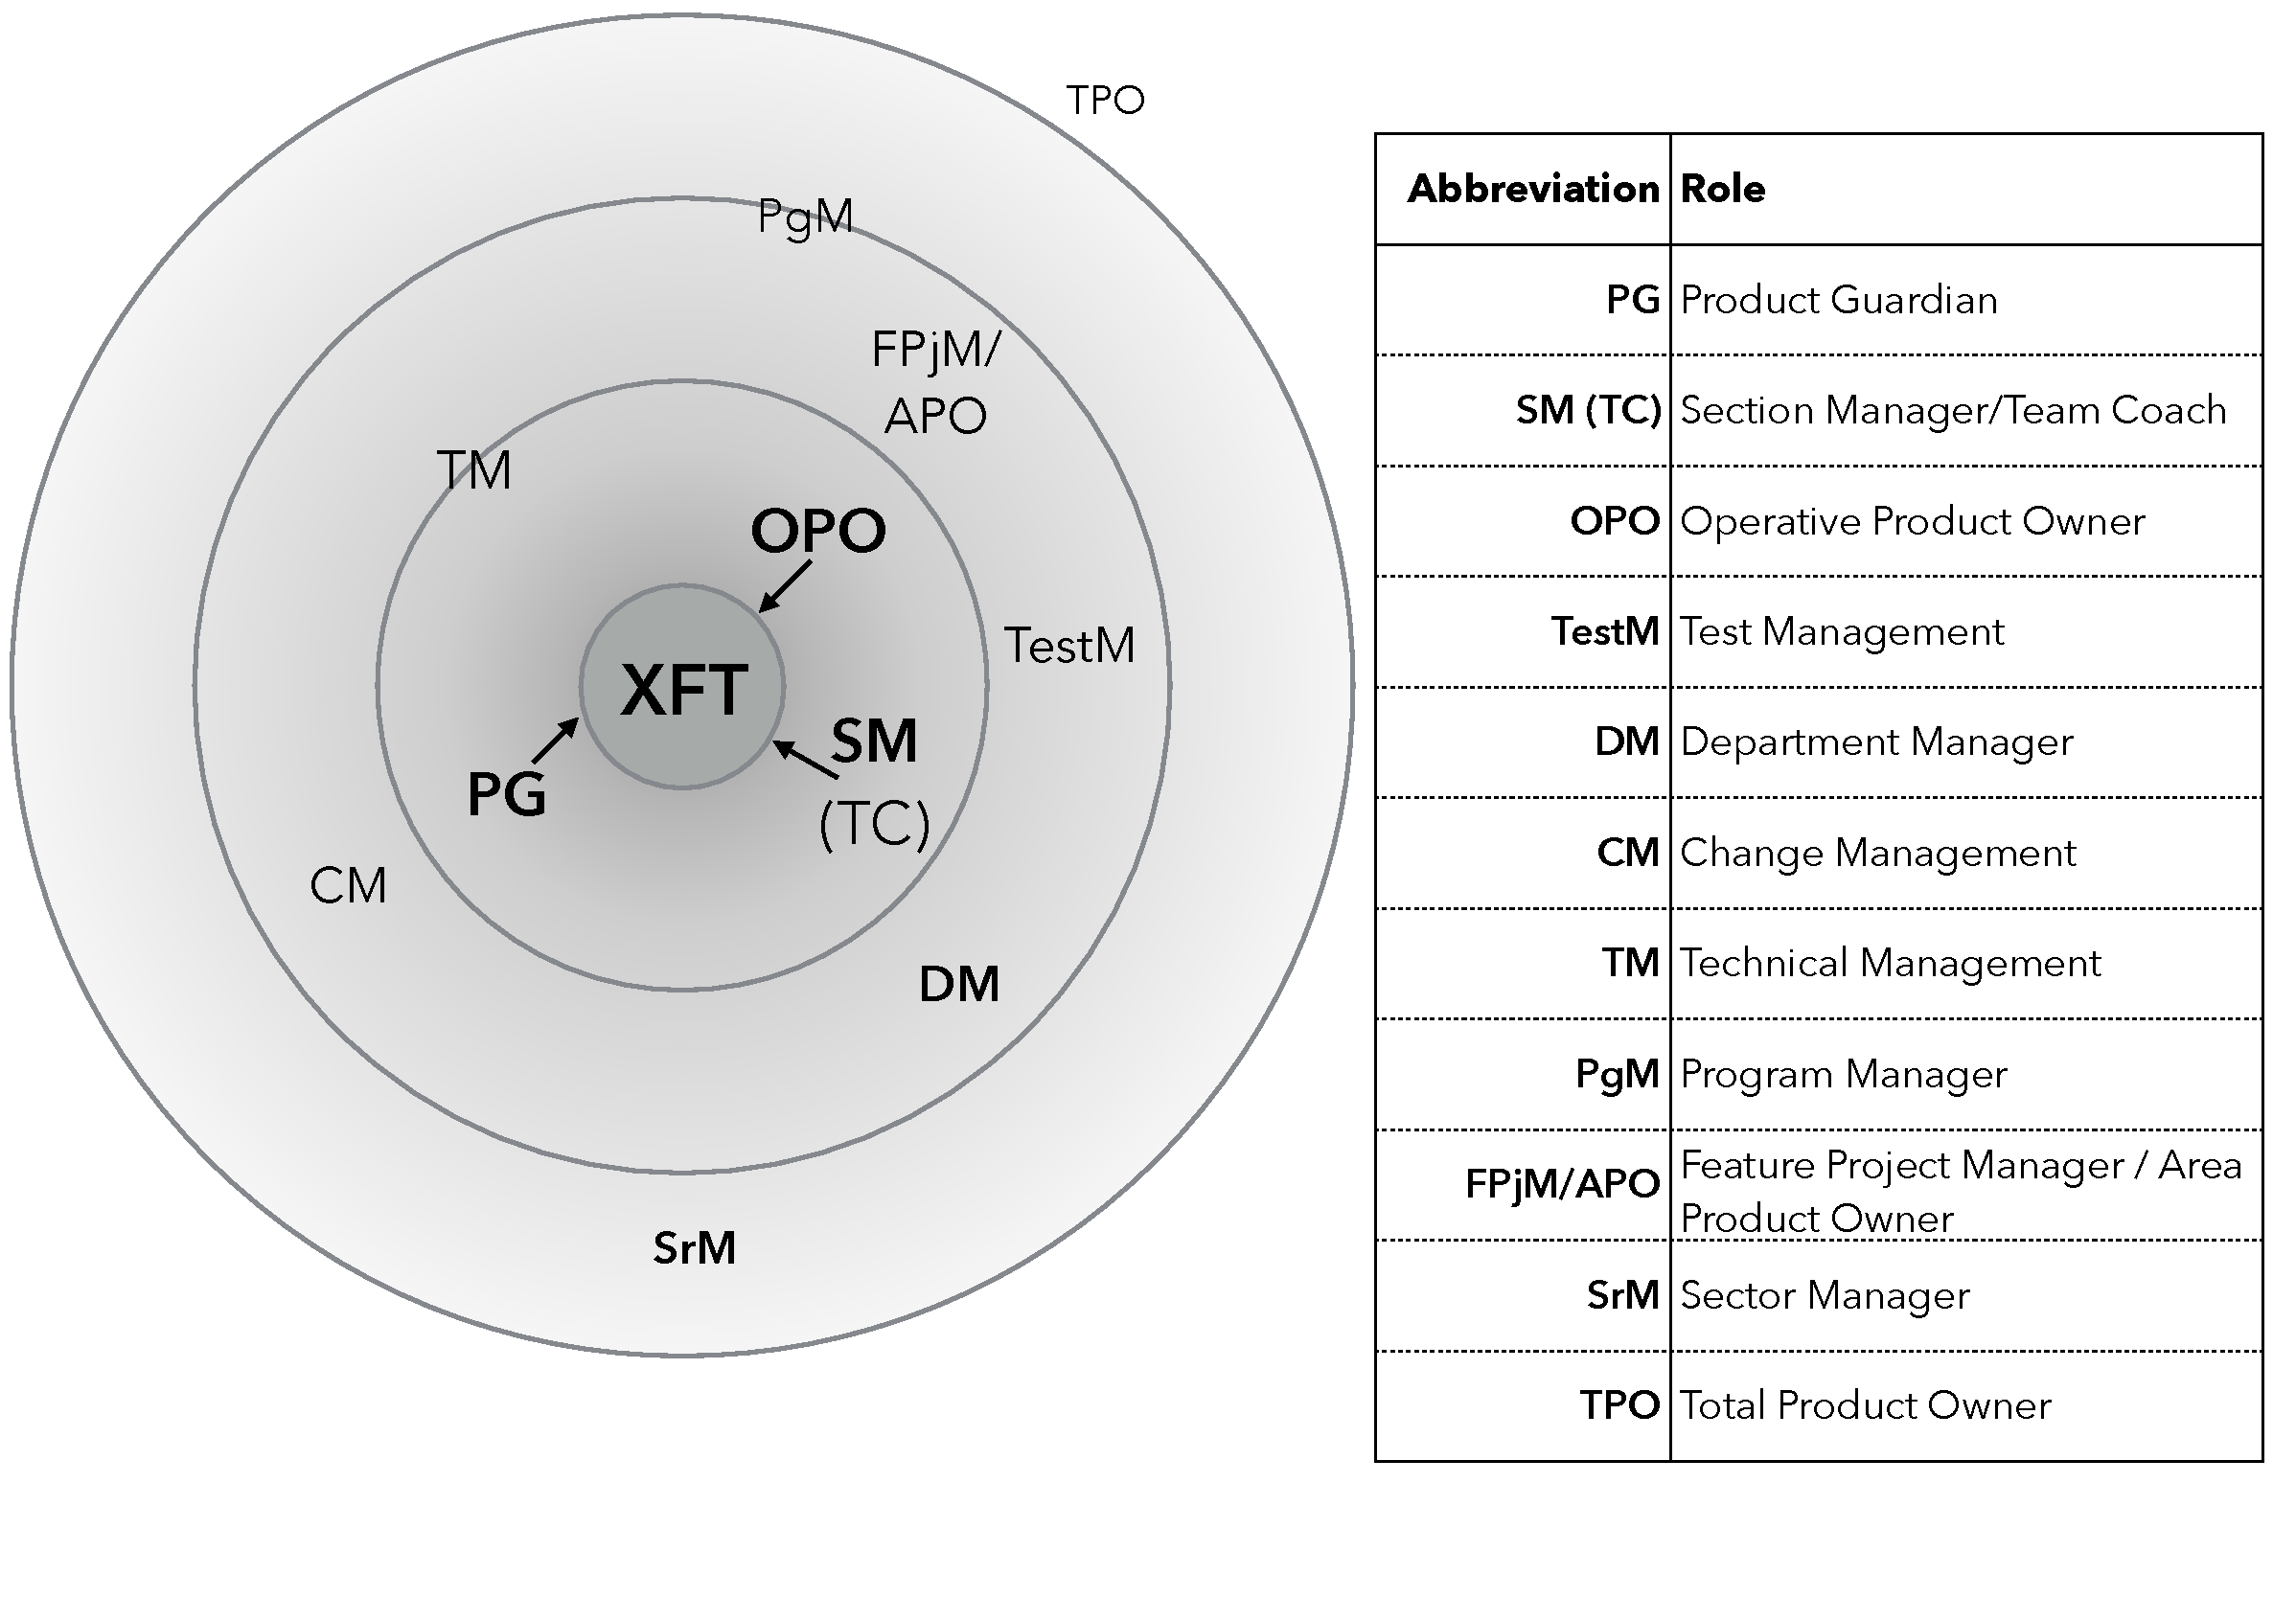
\includegraphics[width=0.8\textwidth]{figures/onion.pdf}
  \caption{Layers of roles and their interaction}
  \label{onion}
\end{figure}

Figure~\ref{onion} illustrates the distance and an intended amount of collaboration between the roles by outlining layers of interaction. An~\ac{XFT} is always in the closest and immediate contact and cooperation with the~\ac{PG} of the product they work on, their~\ac{OPO} and~\ac{SM}. The next layer is comprised of those roles who have a frequent contact to the~\ac{XFT} and their environment while the degree of this contact is significantly lower than in the first layer. Hence, the bigger distance from the~\ac{XFT} to another role, the less communication is envisioned.

\newpage

\subsection{Role Descriptions \& Definitions}

The more detailed description of the roles inside the organisation, including a short description of the key tasks for each, can be found in the table below. %don't ask me why using the ref ain't working 

\begin{table}[h]
   \begin{tabularx}{\textwidth}{ | p{6.9cm} | p{6.9cm} | }
   
   \hline
   \emph{Description} & \emph{Key Tasks} \\ 
   \hhline{==}
   
   \multicolumn{2}{ | c | }{\textbf{Agile Coach}}
   
   \\ \hline
   
   \begin{itemize}[label={}, leftmargin=*, topsep=0pt, itemsep=0pt, partopsep=0pt]
     \item Coaches the organisation in the new ways of working by covering problematic and uncertain areas not handled by the existing organisational roles. Coaches the leadership team and management but also interacts with individual \acp{XFT} and other agilean roles when needed. After the settlement of new ways of working, the responsibilities are handed over to Section Managers. 
   \end{itemize} &
   
   \begin{itemize}[label={}, leftmargin=*, topsep=0pt, itemsep=0pt, partopsep=0pt]
     \item Drive agile and lean improvements in the organisation.
     \item Give feedback on ways to improve working.
     \item Drive workshops and retrospectives related to agile and lean.
     \item Coach teams to improve and become high-performing.
     \item Investigate, find and propose methods to improve teams and organisation.
     \item Participate in meetings when applicable (for Leadership Team, XFT, Program, Community of Practice, etc.).
     \item Work as a bridge between organisations on items related to ways of working and agile and lean.
   \end{itemize}
   
   \\ \hline
   
   \hline
      
   \multicolumn{2}{ | c | }{\textbf{Feature Project Manager}} 
   
   \\ \hline
   
   \begin{itemize}[label={}, leftmargin=*, topsep=0pt, itemsep=0pt, partopsep=0pt]
     \item End-to-end responsible for features/other work items in case of them being too large and complex to be managed by a single \ac{OPO}. Handles related coordination and progress reporting. 
   \end{itemize} & 

   \begin{itemize}[label={}, leftmargin=*, topsep=0pt, itemsep=0pt, partopsep=0pt]
     \item Support \acp{OPO} and teams with planning and coordination (e.g. between OPOs, teams, standards, projects, PDUs etc).
     \item Provide time plans and status updates.
     \item Report the status and escalate issues when needed.
     \item Follow up and reporting.
     \item Represent their part of a complex feature on a bigger scale.
   \end{itemize} 
   
   \\ \hline
   
   \end{tabularx}
\end{table}

\begin{table}[h]
   \begin{tabularx}{\textwidth}{ | p{6.9cm} | p{6.9cm} | }
   
   \hline
   \multicolumn{2}{ | c | }{\textbf{Operative Product Owner (OPO)}}
   
   \\ \hline
   
   \begin{itemize}[label={}, leftmargin=*, topsep=0pt, itemsep=0pt, partopsep=0pt]
     \item Acts as a customer on the site for 2-5 \acp{XFT}, shaping team's backlog. Follows the quality of the developed feature and makes sure its end value is understood by the \ac{XFT}. Involved in technical development aspects, such as integration risks and technical dependencies.
   \end{itemize} & 
   
   \begin{itemize}[label={}, leftmargin=*, topsep=0pt, itemsep=0pt, partopsep=0pt]
     \item Prioritize user stories across backlogs.
     \item Give feedback on end to end time plan.
     \item Handle teams' backlogs and know their status.
     \item Provide delivery time plan and input to check-lists.
     \item Facilitate cross \acp{XFT} learning by diversifying user stories or arranging meetings.
   \end{itemize} 
   
   \\ \hline
      
   \multicolumn{2}{ | c | }{\textbf{Product Guardian (PG)}} 
   
   \\ \hline
   
   \begin{itemize}[label={}, leftmargin=*, topsep=0pt, itemsep=0pt, partopsep=0pt]
     \item Secures product quality by ensuring unity of architecture and code structure within product/domain and alignment to software outside the domain. Knowledgeable within a specified domain of software and uses their skill to support \acp{XFT} and build up competence in the organisation. Actively cooperates with \acp{OPO} on product improvement items to be put into \ac{XFT}'s backlogs.
   \end{itemize} & 
   
   \begin{itemize}[label={}, leftmargin=*, topsep=0pt, itemsep=0pt, partopsep=0pt]
     \item Help in technical decisions related to a product/domain that goes in line with fulfilling the product vision and quality requirements.
     \item Have a vital few design rules for the product.
     \item Support the creation of definition of done for features affecting the product.
     \item Collect and prioritize product care and improvement items.
     \item Coach less experienced people when working with the product's code, documents and test.
   \end{itemize} 
   
   \\ \hline
   
   \hline
   
   \multicolumn{2}{ | c | }{\textbf{Program Manager}}
   
   \\ \hline
   
   \begin{itemize}[label={}, leftmargin=*, topsep=0pt, itemsep=0pt, partopsep=0pt]
     \item Manages the program backlog, which is focused around a group of requirements from the product line.
   \end{itemize} & 
   
   \begin{itemize}[label={}, leftmargin=*, topsep=0pt, itemsep=0pt, partopsep=0pt]
     \item Discuss requirements and their release with the \ac{APO}.
     \item Facilitate program meetings with \acp{OPO} where they pull items from the backlog.
     \item Appoint a Feature Project Manager when main requirements are too much to handle for \acp{OPO}.
   \end{itemize} 
   
   \\ \hline

   \end{tabularx}
\end{table}

\begin{table}[t]
   \label{table:roledefinitions}
   \begin{tabularx}{\textwidth}{ | p{6.9cm} | p{6.9cm} | }
   
   \hline 
   
   \multicolumn{2}{ | c | }{\textbf{Section Manager (SM)}}
   
   \\ \hline 
   
   \begin{itemize}[label={}, leftmargin=*, topsep=0pt, itemsep=0pt, partopsep=0pt]
     \item Combines legal personnel responsibility and support of the \acp{XFT} by removing impediments that the teams cannot handle themselves and helping out with competence planning.  
   \end{itemize} & 
   
   \begin{itemize}[label={}, leftmargin=*, topsep=0pt, itemsep=0pt, partopsep=0pt]
     \item Participate frequently in \ac{XFT}'s stand-ups, demos, backlog preparations.
     \item Give feedback to \acp{XFT} and Scrum Masters.
     \item Involve Scrum Masters in discussions about team set ups, recruitments and processes.
   \end{itemize} 
   
   \\ \hline
   
   \multicolumn{2}{ | c | }{\textbf{Team Coach}} 
   
   \\ \hline
   
   \begin{itemize}[label={}, leftmargin=*, topsep=0pt, itemsep=0pt, partopsep=0pt]
     \item With application of Scrum as an area of expertise, acts as an Agile Coach on a team level typically for 2 \acp{XFT} by e.g. facilitating workshops and introducing methods.
   \end{itemize} & 
   
   \begin{itemize}[label={}, leftmargin=*, topsep=0pt, itemsep=0pt, partopsep=0pt]
     \item Give feedback on ways to improve working.
     \item Drive workshops related to agile and lean questions.
     \item Coach teams to improve and become high-performing.
     \item Investigate, find and propose methods to improve teams and organisation.
     \item Participate in meetings when applicable (for Leadership Team, XFT, Program, Community of Practice, etc).
     \item Handle impediments that the teams can not handle themselves.
   \end{itemize} 
   
   \\ \hline
   
   \multicolumn{2}{ | c | }{\textbf{XFT Scrum Master}}
   
   \\ \hline 
   
   \begin{itemize}[label={}, leftmargin=*, topsep=0pt, itemsep=0pt, partopsep=0pt]
     \item Ensures adherence of the \ac{XFT}'s process to Scrum. Filters interactions from outside to their \acp{XFT} based on their helpfulness. Acts according to a traditional theory concept, encouraging the team to improve its development process.
   \end{itemize} & 
   
   \begin{itemize}[label={}, leftmargin=*, topsep=0pt, itemsep=0pt, partopsep=0pt]
     \item Communicate visions, goals and product backlog items to the \ac{XFT} and assure efficient backlog management techniques.
     \item Coach the \ac{XFT} into self-organisation and cross-functionality.
     \item Lead and coach the team in its Scrum adoption.
     \item Work with other Scrum Masters to increase the effectiveness of the application of Scrum in the organisation.
   \end{itemize} 
   
   \\ \hline

  \end{tabularx}
  \caption{Role descriptions}
\end{table}
